\begin{thmx}{Friedrichs' Inequality}
Let $\Omega$ be contained in a hypercube with sidelength $s$. Then 
\begin{equation*}
    \| v \|_0 \leq s |v|_1 \quad \quad \forall v \in H_0^1(\Omega).
\end{equation*}\label{thm:friedrich}
\vspace{-8mm}
\end{thmx}
\begin{bev}
We will start by assuming $v \in C_0^{\infty}(\Omega)$, and later use the 
completeness of $H_0^1(\Omega)$ to finish the proof.
Let $W = \{ (x_1, \ldots, x_n) \mid 0 < x_i < s \}$ be the box 
which contains $\Omega$, and let $v(x)=0$ \, $\forall x
\in W\setminus \Omega$. Otherwise we can simply translate $\Omega$ such that 
this is true.
 We can then write 
\begin{equation*}
v(x)=v(0, x_2, \ldots, x_n) + \int_{0}^{x_1} \partial _1 v(t,x_2, \ldots, x_n) dt.
\end{equation*}
Due to the definition of $W$, the first term (the boundary term) 
disappears. Applying the Cauchy-Schwartz inequality results in 
\begin{align*}
    |v(x)|^2 &= \left|\int_{0}^{x_1} \partial _1 v(t,x_2, \ldots, x_n) dt \right|^2 \\ 
    &= |{(1, \partial _1 v)}_{L^2([0,x_1])}|^2 \\
    & \leq \int_{0}^{x_1} 1^2 dt \int_{0}^{x_1}|\partial_1 v(t, x_2, \ldots, x_n)|^2 dt \\ 
    &\leq s \int_{0}^{s}|\partial_1 v(t, x_2, \ldots, x_n)|^2 dt. 
\end{align*}
After expanding the integral and getting the last inequality, we know 
the right hand side is independent of $x_1$, and so by integrating we find 
\begin{equation*}
    \int_{0}^{s}|v(x)|^2dx_1 \leq s^2\int_{0}^{s}|\partial _1 v(x)|^2dx_1.
\end{equation*}
This can be done for every variable, and finding the integral over the entire 
domain gives us 
\begin{equation*}
    \|v\|_0 = \int_{W}|v|^2 dx \leq s^2 \int_{W} |\partial _1v|^2 \leq s^2 |v|_1^2.
\end{equation*}
Since $C^\infty_0(\OO)$ is complete in $H_0^1(\OO)$, for every $u \in H_0^1(\OO)\setminus C^\infty_0(\OO)$
there exists some Cauchy sequence of smooth functions $u_k \in C^\infty_0(\OO)$
 such that 
\begin{equation}
    \lim_{k \to \infty} \| u-u_k\|_1 \to 0.
    \label{eq:friedrich_cauchy_limit}
\end{equation}
We have proven Theorem~\ref*{thm:friedrich} for every one of these $u_k$, and 
since $s^2$ is independent of $k$, we can write 
\begin{equation*}
    \|u\|_0 \leq \|u_k\|_0 + \|u-u_k\|_0 \leq  s^2|u_k|_1 +  \|u-u_k\|_0 \leq s^2|u|_1 + s^2|u-u_k|_1 + \|u-u_k\|_0.
\end{equation*}
By (\ref*{eq:friedrich_cauchy_limit}), both of the last terms in the 
previous equation must tend to $0$ as $k \to \infty$, and we have the proof.
\end{bev}
Theorem~\ref{thm:friedrich} and Corollary~\ref{cor:friedrich_n} both deal with 
functions which are zero on the boundary. 
This is restrictive, and we would like to be able to examine 
functions which are not zero on the boundary.
To remedy this, we introduce the Trace Theorem, which requires the cone condition, which we now define.
\begin{defn}{Cone}
    
\end{defn}






\begin{defn}{Cone Condition}~\label{def:cone_condition}
    Let $E$ be a Euclidean space and let $G$ be an open subset of $E$.
    Let $\varepsilon >0$, and define 
    $V(w, l)$ to be a cone with vertex at origo, opening $\varepsilon$, axis $w$,
    and height $l$.
    Also define $\mathcal{E} = \{e(g) | g \in G, \, e(g) \text{ is a straight line}\}$ 
    to be the set of all possible straight lines going through each point in $G$. %Kan det misfortåes? Linjen skal ikke gå gennem alle, men et specifikt punkt.
    The cone condition is defined to be: %FIXME Formel for cone
    \begin{equation*}
        \exists h \leq \infty \,\,
        %\exists e\in \mathcal{E} \,\, : \,\,  \forall x \in G \implies 
        \forall x \in G\,\, \exists e\in \mathcal{E} \,\, :
        x + V(e(x), h) \subset G. % + er translation
    \end{equation*}
    This means: at all points in $G$, we can create a cone with positive opening,
    with some height, pointing in some direction, such that the cone is contained 
    in $G$.
\end{defn}
\begin{figure}[H]
    \centering
    \begin{subfigure}{.3\textwidth}
        \centering
        \begin{tikzpicture}
	\path[draw=black, line width =1pt, line join=round]  (0,0) .. controls (-0.2,1.5) .. (1,1)
		-- (1.5,1) .. controls (1,0) .. (1.2,-0.2)
		.. controls (1.5,-1.5) .. (-0.25,-1)
		.. controls (-0.5, -0.5) .. cycle;
  \node [isosceles triangle,
         isosceles triangle apex angle=20,
         rotate = 30,
         fill=gray!25,
         anchor=apex,
         minimum width=2pt] (t) at (1.5,1) {};    
\end{tikzpicture}
        \caption{Space which fulfill the Cone Condition}~\label{fig:cone_condition_true}
      \end{subfigure}
    \begin{subfigure}{.3\textwidth}
        \centering
        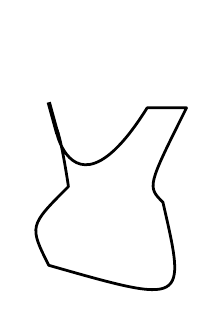
\begin{tikzpicture}
	\path[draw=black, line width =1pt, line join=round]  (0,0) .. controls (-0.3,2) and 
		(-0.25, -1) .. (1,1)
		-- (1.5,1) .. controls (1,0) .. (1.2,-0.2)
		.. controls (1.5,-1.5) .. (-0.25,-1)
		.. controls (-0.5, -0.5) .. cycle;
	\path[draw=black, line width = 1.5pt, line join=round] (-0.14,0.67) -- (-0.25,1.07);
\end{tikzpicture}
        \caption{Space which does not fulfill the Cone Condition}~\label{fig:cone_condition_false}
      \end{subfigure}
      \caption{The Cone Condition visualized}~\label{fig:cone_condition_visu}
\end{figure}
In Figure~\ref{fig:cone_condition_visu}, two spaces are visualized.
 The space in Figure~\ref{fig:cone_condition_true} fulfills the Cone Condition as seen 
 by the grey cone, which can be translated, rotated and scaled to any point, and still 
 be contained in the space. The space  
 in Figure~\ref{fig:cone_condition_false} does not fulfill the Cone Condition, as
in the upper left section of the space a cone cannot be drawn.


With Definition~\ref{def:cone_condition}, we can proceed to the Trace Theorem.
\begin{thmx}{Trace Theorem}~\label{thm:trace}
    Let $\Omega$ be a bounded, and suppose $\Omega$ has a piecewise smooth boundary. In addition, suppose $\Omega$ satisfies the cone condition. Then there exists a bounded linear mapping 
    \begin{equation*}
        \gamma : H^1(\Omega) \to L_2(\partial \Omega)
    \end{equation*}
\end{thmx}
\begin{bev}
    The presented proof will only be done in two dimensions, but can be generalised to higher dimensions.
    Suppose the boundary is piecewise smooth, and for the finitely many points where the boundary is not smooth the cone condition is satisfied. We can split the boundary into a finite number of smooth pieces $\partial \Omega_1, \partial \Omega_2, \dots, \partial \Omega_m$, where each $\partial \Omega_i$ after rotation of the coordinate system gives us
    \begin{enumerate}
        \item For some function $\phi = \phi_i \in C^1[y_1, y_2]$, we have
            \[ \Gamma_i = \{ (x,y) \in \RR^2 \quad | \quad x = \phi(y), y_1 \leq y \leq y_2 \}. \]
        \item The domain $\Omega_i = \{ (x,y) \subset \RR^2 \quad | \quad \phi(y) < x <\phi(y) + r, y_1 < y < y_n \}$ is contained in $\Omega$, where $r > 0$ is sufficiently small. 
    \end{enumerate}
    Firstly a function $v \in C^1(\bar{\Omega})$ and a point $(x,y) \in \partial \Omega$ can be written as
    \begin{equation}
            v(\phi(y), y) = v(\phi(y) + t, y) - \int_0^t \partial_1 v(\phi(y) + s, y) \, ds~\label{eq:trace_integral}
    \end{equation}
    where $0 \leq t \leq r$. By integrating~\eqref{eq:trace_integral} and switching the integration order we obtain 
    \begin{align*}
        \int_0^r v(\phi(y), y) dt &= \int_0^r \left(   v(\phi(y) + t, y) - \int_0^t \partial_1 v(\phi(y) + s, y) \, ds \right) dt \\
        r v(\phi(y), y) dt &= \int_0^r   v(\phi(y) + t, y) dt - \int_0^r \int_0^t \partial_1 v(\phi(y) + s, y) \, ds dt \\
        r v(\phi(y), y) dt &= \int_0^r   v(\phi(y) + t, y) dt - \int_0^r \int_s^r \partial_1 v(\phi(y) + s, y) \, dt ds \\
        r v(\phi(y), y) dt &= \int_0^r v(\phi(y) + t, y) dt - \int_0^r \partial_1 v(\phi(y) + t, y)(r-t) dt.
    \end{align*}
    By squaring the former equation, using a form of Young's inequality ${(a+b)}^2 \leq 2a^2 + 2b^2$, and appply the Cauchy-Schwarz inequality to the squares of the integrals results in
    \begin{equation}
        r^2 v^2(\phi(y), y) \leq 2 \int_0^r 1 dt \int_0^r v^2(\phi(y) + t, y) \, dt +  2\int_0^r t^2 \int_0^r | \partial_1  v(\phi(y) + t, y) |^2 dt
    \end{equation}
    By subsituting $\int 1 dt = r$ and $\int t^2 dt = \frac{r^3}{3}$, dividing by $r^2$ and integrating over $y$, we obtain
    \begin{align*}
        \int_{y_1}^{y_2} v^2(\phi(y), y) dy &\leq  2r^{-1} \int_{\Omega_i} v^2 dx dy + \frac{2r}{3} \int_{\Omega_i} | \partial_1 v |^2 dx dy \\
        &\leq  2r^{-1} \int_{\Omega_i} v^2 dx dy + r \int_{\Omega_i} | \partial_1 v |^2 dx dy 
    \end{align*}
    On $\partial\Omega$ the arc length differential is given by $ds = \sqrt{1 + \phi'{(y)}^2} dy$. Thus, we have
    \begin{equation}
        \int_{\partial\Omega} v^2 ds \leq c_i \left[ 2r^{-1} \| v \|_0^2 + r | v |^2_1 \right],
    \end{equation}
    Where $c_i = \text{max}\{\sqrt{1+{\phi'}^2} | y_1 \leq y \leq y_2 \}$. Setting $c=(r+2r^{-1})\sum_{i=1}^m c_i$, results in
    \begin{equation}
        \| v \|_{0,\partial\Omega} \leq c \| v \|_{1,\Omega}.
    \end{equation}
    Thus, the restriction $\gamma : H^1(\Omega) \cap C^1(\bar{\Omega}) \to L_2(\partial \Omega)$ is a bounded linear mapping on a dense subset of $H^1(\OO)$. Because of the completness of $L_2(\partial \Omega)$, it can be extended to all of $H^1(\Omega)$ without enlarging the bound.
\end{bev}
Theorem~\ref{thm:trace} guarantees that functions which are not 
zero on the boundary are at least an $L_2$ function, and as such are bounded. 
\subsection{Attributes of Solutions}
In this section we examine certain qualities of solutions, and the first step is 
the ability to characterize solutions to certain problems.
To do that, we introduce the following theorem.

\begin{thmx}{Characterization Theorem}
\label{thm:charac_theorem}
    Let $V$ be a linear subspace, such that
        \[
            a: VxV \rightarrow \mathbb{R}
        \]
    is a symmetric positive bilinear form, then $a(v,v)>0$ for all $v \in V$, $v \neq 0$. In addition, let
        \[
            \ell: V \rightarrow \mathbb{R}
        \]
    be a linear functional. Then the quantity

        \[
            J(v):=\frac{1}{2} a(v,v) - \langle\ell,v\rangle 
        \]
    optains its minimum over $V$ at $u$ if and only if
        \begin{equation}
        \label{eq:charac}
            a(u,v) = \ell(v) \quad \text{for all } v \in V.
        \end{equation}
    There is at most one solution to~\eqref{eq:charac}.
\end{thmx}

\begin{proof}

    For $u,v \in V$ and $t \in \mathbb{R}$ we have, that
    \begin{align}
        J(u+tv) &= \frac{1}{2} a(u+tv,u+tv) - \langle\ell,u+tv\rangle \nonumber \\
        &= \frac{1}{2} \left( a(u,u) + a(tv,tv) + 2a(u,tv) \right) - \left( \langle \ell,u\rangle + \langle\ell,tv\rangle \right) \nonumber \\
        &= J(u) + t\left( a(u,v) - \langle\ell,v\rangle \right) + \frac{1}{2}t^2a(v,v). \label{eq:charac_proof_J(u+tv)}
    \end{align}

    If $u \in V$ satisfies~\eqref{eq:charac} and $t=1$, then from~\eqref{eq:charac_proof_J(u+tv)} we have, that
    \begin{alignat}{2}
        J(u+v) &= J(u) + \frac{1}{2}a(v,v) \quad &&\text{for all } v\in V  \nonumber \\
        &> J(u) \quad &&\text{for } v \neq 0.
    \end{alignat}
    Thus $u$ is a ubnique minimal point. 

    To prove the opposite way, we assume that $J$ has a minimum at $u$, then for every $v\in V$, the derirative of the function $t \mapsto J(u+tv)$ must vanish at $t=0$. 
    By~\eqref{eq:charac_proof_J(u+tv)} the derirative of $J(u+tv)$ with respect to $t$ can be found using, that
    \begin{align*}
          J(u+(t+h)v) &= J(u) + (t+h) (a(u,v) - \langle \ell,v\rangle) + \frac{1}{2}(t+h)^2 a(v,v) \\
          &= J(u+tv) + h(a(u,v) - \langle \ell,v\rangle) + \frac{1}{2}((h^2+2th)a(v,v)),
    \end{align*}
    thus the derirative is $a(u,v) - \langle \ell,v\rangle$, and~\eqref{eq:charac} then follows.
\end{proof}
To use Theorem~\ref{thm:charac_theorem}, we
only make assumptions on the linearity of the space, however we
do not guarantee the existence  of solutions, only their characterization.
It is possible to set up a variational problem such that $J$ does 
not attain its minimum.
To engage with the existence of solutions, we make more assumptions on 
the space in which we work.
We start by specifying the bilinear form in Theorem~\ref{thm:charac_theorem}.
\begin{defn}{\quad}
   Let $H$ be a Hilbert space. A bilinear form $a : H \times H \to \RR$ is 
   called continuous if there exists some $C > 0$ such that 
   \begin{equation}
    |a(u,v)| \leq C \|u\|\, \|v\| \quad \forall u,v \in H.
   \end{equation} 
   If a bilinear form $a$ is symmetric and continuous, and there exists som $\alpha >0$ such that 
   \begin{equation*}
    a(v,v) \geq \alpha \|v\|^2 \quad \forall v \in H,
   \end{equation*}
   $a$ is called elliptic.\label{def:elliptic}
 \end{defn}
From this point forward $a$ will be referring to the bilinear form given by
\begin{equation}
   a(u,v) = \int_\Omega \left[\sum_{i,k} a_{ik}\partial_i u\partial_k v+a_0uv\right]dx,
\end{equation}
unless otherwise stated.
%FIXME Beskriv hvorfor en elliptic diff operator giver en elliptic a

\section{Homogeneous Dirichlet Conditions}
Since we are trying to solve the PDE over some space $\Omega$, we write
\begin{align}
\begin{split}
    Lu &= f \quad \text{in } \Omega \label{eq:b_v_problem} \\
    u &= g \quad \text{on } \partial \Omega.
\end{split}
\end{align}
A boundary condition on the form~\eqref{eq:b_v_problem} is called a 
Dirichlet condition, which is when $u$ itself is specified on the boundary. 
If $u=0$ on the boundary we have homogeneous boundary conditions, which we usually assume 
to make things easier. If that is not the case, we can
transform the problem. To do this, we assume there exists a function 
$\tilde{u}$ such that $\tilde{u}=g$ on $\partial \Omega$. Then we define 
$w = u - \tilde{u}$ and $\tilde{f}=f-L\tilde{u}$ and we get that
\begin{align}
\begin{split}
    Lw &= \tilde{f} \quad \text{in } \Omega \label{eq:b_v_problem_homogeneous} \\
    w &= 0 \quad \text{on } \partial \Omega. 
\end{split}
\end{align}
To make these explicit demands for $u$ on $\partial \OO$ can 
be rather restrictive.
Instead we can make implicit restrictions, by constraining 
$\partial _i u$ on $\partial \OO$.
This will be dealt with later.

We now use Theorem~\ref{thm:charac_theorem} to show a link between classical 
solutions and solutions of appropriate variational problems.
\begin{thmx}{Minimal Property}
    Every classical solution of the boundary-value problem, given by
\begin{align}
    -\sum_{i,k} \partial_i (a_{ik}\partial_k u) + a_0 u &= f \quad \text{in } \Omega  \\
    u &= 0 \quad \text{on } \partial \Omega,
\end{align}
    is a solution to the variational problem, given by
    \[
        J(v)=\int_\Omega \left [\frac{1}{2}\sum_{i,k} a_{ik} \partial_i v\partial_k v + \frac{1}{2} a_0 v^2 -fv\right ]dx \longrightarrow \min,
    \]
    among all functions in $C^2(\Omega)\cap C^0(\bar{\Omega})$ with zero boundary values. 
\end{thmx}
\begin{proof}
    We start off by applying Green's formula
    \begin{equation}
    \label{eq:Greens_formula}
        \int_\Omega v\partial_i w dx = -\int_\Omega w \partial_i v dx + \int_{\partial \Omega} v w \vec{n}_i ds.
    \end{equation}
    Here we assume $v$ and $w$ to be $C^1(\OO)$ functions, and $\vec{n}_i$ is the $i$'th component of the outward-pointing normal $\vec{n}$.
    Now if we insert $w=a_{ik}\partial_k u$ in~\eqref{eq:Greens_formula}, we get
    \begin{equation}
    \label{eq:Greens_formula_inserted}
        \int_\Omega v\partial_i (a_{ik} \partial_k u) dx = -\int_\Omega a_{ik} \partial_i v v\partial_k u dx,
    \end{equation}
    given that $v=0$ on $\partial \Omega$.
    Now let 
    \begin{equation}
    \label{eq:a(u,v)}
        a(u,v) = \int_\Omega \left[\sum_{i,k} a_{ik} \partial_i u \partial_k v +a_0 uv \right]dx
    \end{equation}
    and
    \begin{equation}
    \label{eq:l(v)}
        \ell(v) = \int_\Omega fv dx.
    \end{equation}
    Then by summing~\eqref{eq:Greens_formula_inserted} over $i$ and $k$ we get that for every $v\in C^1(\Omega) \cap C(\bar{\Omega})$ with $v=0$ on $\partial \Omega$ we have
    \begin{align}
        a(u,v) - \ell(v) &= \int_\Omega v\left[ -\sum_{i,k} \partial_i (a_{ik} \partial_k u) + a_0 u - f \right] dx \label{eq:min_prop_variational_problem}\\
        &= \int_\Omega v [Lu - f] dx \nonumber \\
        &= 0, \nonumber
    \end{align}
    given that $Lu = f$. This property holds if $u$ is a classical solution.
     The minimal property is then implied by Theorem~\ref{thm:charac_theorem}
\end{proof}
The same kind of proof can be used to show that a solution $u$ to~\eqref{eq:min_prop_variational_problem} which fulfills 
$u\in C^2(\OO) \cap C^0(\OO)$ is also a classical solution. 
When $u\in C^2(\OO) \cap C^0(\OO)$ the variational problem and 
homogeneous boundary value problem are thusly equivalent.
We can therefore use the variational problem to find solutions, making the
 the following theorem useful.
\begin{thmx}{Lax-Milgram Theorem}
Let $V$ be a closed, convex, non-empty set in a Hilbert space $H$, and let $a:H \times H \rightarrow \mathbb{R}$ be an elliptic bilinear form. Then for every $\ell\in H'$, the variational problem given by
\[
    J(v)=\frac{1}{2} a(v,v) - \ell(v) \longrightarrow \min    
\]
has a unique solution in $V$.\label{thm:lax_milgram}
\end{thmx}

\begin{bev}
    $J$ is bounded from below, since
    \begin{align*}
        J(v) &\geq \frac{1}{2} \alpha \|v\|^2 - \|\ell\| \, \|v\|\\
        &= \frac{1}{2\alpha} {(\alpha \|v\|-\|\ell\|)}^2 - \frac{\|\ell\|^2}{2\alpha} \\
        &\geq - \frac{\|\ell\|^2}{2\alpha}.
    \end{align*}
    We then let $c_1 = \inf\{J(v); v \in V\}$ and ${\{v_n \}}_{n=1}^\infty$ be a minimizing sequence. Then we get 
    \begin{align*}
        \alpha \|v_n-v_m\|^2 &\leq a(v_n-v_m,v_n-v_m) \\
        &= 2a(v_n,v_n) + 2a(v_m,v_m) - a (v_n+v_m,v_n+v_m) \\
        &= 4J(v_n) + 4J(v_m) - 8J(\frac{v_m+v_n}{2}) \\
        &\leq 4J(v_n) + 4J(v_m) - 8c_1. 
    \end{align*}
    By the convexity assumption on $V$, we get that $\frac{1}{2}(v_n + v_m) \in V$, and from that we get the last 
    inequality.
    We now get that ${\{v_n \}}_{n=1}^\infty$ is a Cauchy sequence in $H$ and $u = \lim_{n\rightarrow \infty}v_n$ exists given the fact that $J(v_n),J(v_m)\rightarrow c_1$ implies $\|v_n - v_m\| \rightarrow 0$ for $n,m\rightarrow \infty$.  

    Since $J$ is continuous,
    we see $J(u) = \lim_{n\rightarrow \infty} J(v_n) = \inf_{v\in V} J(v)$.
     Moreover, we also have that $u\in V$, because we assumed $V$ to be closed. 
    Lastly, we need to show that the solution is unique.
     To do that, we assume both $u_1$ and $u_2$ to be solutions of the variational problem. 
    Then we set up a minimizing sequence $u_1,u_2,u_1,u_2,\ldots$, which we know to be a Cauchy sequence from earlier.
     This implies $u_1 = u_2$.
\end{bev}
As all Hilbert spaces are vector spaces, they will be convex by definition in addition we will limit ourselves to complete Hilbert spaces.
As such, subsets of Hilbert spaces we are going to be working will be as well,
and we can use the following corollary.
We can therefore make use of the following corollary to unify our approach.
\begin{kor}{\quad}
   Assume the same as in Theorem \ref{thm:lax_milgram}, except $V=H$. Then 
   the solution $u$ is given by 
   \label{cor:lax_milgram}
   \begin{equation*}
    a(u,v) = \ell(v).
   \end{equation*}
   \vspace{-9mm}
\end{kor}
\begin{bev}
    The proof follows closely the proof for Theorem \ref{thm:lax_milgram}. 
    Simply replace $V$ with $H$, to find the existence and uniqueness of the 
    solution, and use Theorem \ref{thm:charac_theorem} to find the form, as 
    shown in the corollary.
\end{bev}
Theorem \ref{thm:minimal_property}, Theorem \ref{thm:lax_milgram} and Corollary 
\ref{cor:lax_milgram} together shows us, that solving a Dirichlet problem is 
the same as finding the minimum of the corresponding variational problem. 
We can use this in our approach, both theoretically, and computationally.

When working with PDE's the equation shown in Corollary~\ref{cor:lax_milgram} 
is called the variational formulation of a boundary condition problem. 
To find the solution $u$, we split a Hilbert space of functions, $H$, 
into finite dimensional subspaces, and use these to approximate $u$. 
We test this approximatation using test functions, typically from the same subspace,
 using the equality in Corollary~\ref{cor:lax_milgram}, which must be true for all test functions.
This widens the 
space in which we look for solutions.
For example, by using the variational formulation, we can define a weak solution 
which no longer requires $u \in C^2(\OO)$.
\begin{defn}{\quad}
    A function $u\in H_0^1(\OO)$ is called a weak solution of 
    the Dirichlet problem with homogeneous boundary conditions,~\eqref{eq:b_v_problem_homogeneous}, if 
     \begin{equation*}
        a(u,v) = {(\tilde{f},v)}_0 \quad \forall v \in H_0^1(\OO).
     \end{equation*}
     Here $a(u,v)$ is the bilinear from from~\eqref{eq:a(u,v)}, 
     and ${(\tilde{f},v)}_0$ is a linear bounded functional provided $\tilde{f}\in L^2$, and it can therefore be used as $\ell(v)$ in~\eqref{eq:l(v)}.
\end{defn}
A weak solution only requires $u\in H_0^1(\OO)$, and is clearly less strict. 
Thus there is a higher chance of a solution existing for any given problem, 
and is therefore desirable. So we now look at the existence of weak solutions.
\begin{thmx}{Existence theorem}
    Let $L$ be a second order uniformly elliptic partial differential operator from~\eqref{eq:Lu}. Then the homogeneous Dirichlet problem,
     (\ref{eq:b_v_problem_homogeneous}), always has a weak solution in $H_0^1(\OO)$. It is a minimum of the variational problem
    \begin{equation}
        \frac{1}{2} a(v,v) - {(f, v)}_0 \rightarrow \text{min}
    \end{equation}
    over $H_0^1(\OO)$.\label{thm:existence_hom_dirichlet}
\end{thmx}

\begin{bev}
    Let $c = \sup\{\left| a_{ik}(x) \right| \; | \; x \in \OO, 1 \leq i,k \leq n\}$. Then by the Cauchy-Schwarz inequality we get
    \begin{align}
    \begin{split}
        \left| \sum_{i,k} \int a_{ik} \partial_i u \partial_k v dx \right| &\leq c \sum_{i,k} \int  \left|  \partial_i u \partial_k v dx\right|\\
        &\leq c \sum_{i,k} {\left[ \int {\left( \partial_i u \right)}^2 dx \int {\left( \partial_k v \right)}^2 dx  \right]}^{1/2} \\
        &\leq C {\left| u \right|}_1 {\left| v \right|}_1 \label{eq:Cuv}
    \end{split}
    \end{align}
    where $C=cn^2$. 
    We also assume $C\geq \sup\{|a_0(x)| \; | \; x\in \Omega\}$ giving us
    \begin{equation}
        \left|\int a_0 u v dx \right| \leq C \int |u v| dx \leq C \|u\|_0 \|v\|_0.  
        \label{eq:estimate_a_0}   
    \end{equation}
    Then by~\eqref{eq:Cuv} and~\eqref{eq:estimate_a_0} we get continuity of $a$.
    Furthermore the uniform ellipticity implies the pointwise estimate %TODO Hvorfor gør den det?
    \[
        \sum_{i,k} a_{ik} \partial_i v \partial_k v \geq \alpha \sum_i {\left( \partial_i v \right)}^2,
    \]
    for $\text{C}^1(\OO)$ functions. Integrating both sides and using $\text{a}_0 \geq 0$ leads to %TODO Er det fordi man fjerner noget i integralet?
    \begin{equation}
        a(v,v) \geq \alpha \sum_i \int_\OO {\left(\partial_i v\right)}^2 dx = \alpha |v|^2_1, \quad \forall v \in H^1(\OO).
        \label{eq:alpha_ellipticity}
    \end{equation}
    %TODO ref Friedrich equivalent
    We know from Friedrichs' Inequality $|\cdot|_1$ and $\| \cdot \|_1$ are equivalent norms on $H_0^1$,
     resulting in $a$ being an $H^1$-elliptic bilinear form on $H_0^1(\OO)$.
    From Theorem~\ref{thm:lax_milgram} there exists a unique weak solution which is also a solution of the variational problem.
\end{bev}

%TODO Skriv eksempel der kan udvides til inhomogen, og tilhørende tekst

\section{Inhomogeneous Dirichlet Conditions}
The theory in the previous section have been regarding homogeneous 
Dirichlet problems. However, as mentioned before, inhomogeneous
Dirichlet problems can be turned into homogeneous Dirichlet problems 
using Theorem~\ref{thm:existence_hom_dirichlet}. 
Recall the inhomogeneous Dirichlet problem, Equation~\eqref{eq:b_v_problem}, and let 
$\tilde{u} \in C^2(\OO)\cap C^0(\bar{\OO}) \cap H^1(\OO)$ be a function such that 
\begin{equation*}
   \tilde{u} = g \quad \text{on } \partial \OO,
\end{equation*}
and $w = u-\tilde{u}$ and $\tilde{f} = f-L\tilde{u}$. We now have the homogeneous 
Dirichlet problem 
\begin{align}
\begin{split}
    Lw &= \tilde{f} \quad \text{in } \Omega,  \\
    w &= 0 \quad \text{on } \partial \Omega. 
\end{split}
\end{align}
By Theorem~\ref{thm:existence_hom_dirichlet},
 a weak solution $w \in H_0^1(\OO)$ exists. As ${(L\tilde{u},v)}_0 = a(\tilde{u},v)$,
we get
\begin{alignat*}{2}
      a(w,v) &= {(\tilde{f},v)}_0 \quad &&\forall v \in H_0^1(\OO) \\
      a(u-\tilde{u},v) &= {(f-L\tilde{u},v)}_0 &&\\
      a(u,v) - a(\tilde{u},v) &= {(f,v)}_0 - {(L\tilde{u},v)}_0 \quad && \\
      a(u,v) &= {(f,v)}_0. &&
\end{alignat*}
We stil have the condition $u-\tilde{u}=w\in H_0^1(\OO)$, and the weak formulation 
of the inhomogeneous Dirichlet boundary condition can then be written as
\begin{align*}
   a(u,v) = {(f,v)}_0 \quad \forall v &\in H_0^1(\OO) \\
   u-\tilde{u} & \in H_0^1(\OO).
\end{align*}
By Theorem~\ref{thm:c_dense_in_h}, $C^2(\OO)\cap H^1(\OO)$ is dense in $H^1(\OO)$, 
and $C^0(\bar{\OO})\cap H^1_0(\OO)$ 
is dense in $H^1_0(\OO) \subset H^1(\OO)$. Following the same density arguments 
as have been done several times before, it suffices to look at $\tilde{u}\in H^1(\OO)$, however it is not always possible to find an admissible $\tilde{u}$.

As seen in the two previous sections, a Dirichlet condition on the boundary 
directly prescribe the solution. We cannot always guarantee  
the behaviour of the function on the boundary and thus the Dirichlet condition 
can be too restrictive.
A less restrictive requirement deals with the derivatives on the boundary, 
which the next section will deal with.